\documentclass{whiteboard}
\begin{document}
\begin{frame}[plain,t]
\bbcover{Combinadores}{Introdução}{Prof. Edson Alves}{Campus UnB Gama: Faculdade de Ciências e Tecnologias em Engenharia}

\end{frame}
\begin{frame}[plain,t]
\begin{tikzpicture}
\node[draw,opacity=0] at (0, 0) {x};
\node[draw,opacity=0] at (14, 8) {x};

	\node[anchor=west] (title) at (0.0, 7.0) { \Large \bbbold{Moses Schönfinkel} };

	\node[] (moses) at (3.0, 4.0) { 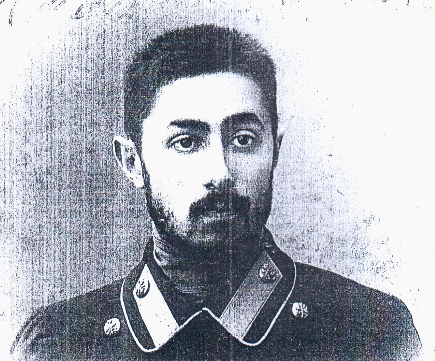
\includegraphics[scale=0.3]{figs/moses2.png} };

	\node[anchor=west] (flag) at (1.2, 1.5) { 
\includegraphics[scale=0.015]{figs/ucrania.png} };

	\node[] (dates) at (3.5, 1.5) { * \bbtext{1889} \hspace*{0.05in} \bbtext{\textdagger\ 1942} };

\end{tikzpicture}
\end{frame}
\begin{frame}[plain,t]
\begin{tikzpicture}
\node[draw,opacity=0] at (0, 0) {x};
\node[draw,opacity=0] at (14, 8) {x};

	\node[anchor=west] (title) at (0.0, 7.0) { \Large \bbbold{Moses Schönfinkel} };

	\node[] (moses) at (3.0, 4.0) { 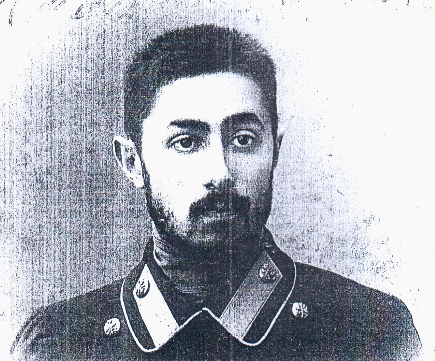
\includegraphics[scale=0.3]{figs/moses2.png} };

	\node[anchor=west] (flag) at (1.2, 1.5) { 
\includegraphics[scale=0.015]{figs/ucrania.png} };

	\node[] (dates) at (3.5, 1.5) { * \bbtext{1889} \hspace*{0.05in} \bbtext{\textdagger\ 1942} };


	\node[anchor=west] (article) at (6.0, 6.0) { \large {\bbnote{On the building blocks of mathematical logic}} };

\end{tikzpicture}
\end{frame}
\begin{frame}[plain,t]
\begin{tikzpicture}
\node[draw,opacity=0] at (0, 0) {x};
\node[draw,opacity=0] at (14, 8) {x};

	\node[anchor=west] (title) at (0.0, 7.0) { \Large \bbbold{Moses Schönfinkel} };

	\node[] (moses) at (3.0, 4.0) { 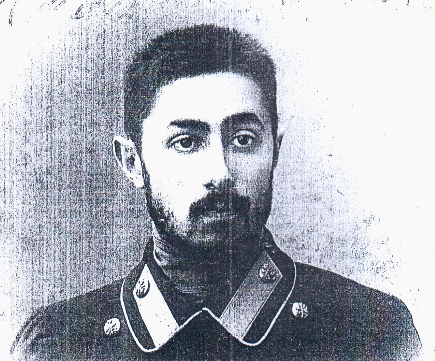
\includegraphics[scale=0.3]{figs/moses2.png} };

	\node[anchor=west] (flag) at (1.2, 1.5) { 
\includegraphics[scale=0.015]{figs/ucrania.png} };

	\node[] (dates) at (3.5, 1.5) { * \bbtext{1889} \hspace*{0.05in} \bbtext{\textdagger\ 1942} };


	\node[anchor=west] (article) at (6.0, 6.0) { \large {\bbnote{On the building blocks of mathematical logic}} };


	\node[anchor=west] (a) at (6.5, 5.0) { $\star$ \bbtext{As ideias foram apresentadas em 1920} };

\end{tikzpicture}
\end{frame}
\begin{frame}[plain,t]
\begin{tikzpicture}
\node[draw,opacity=0] at (0, 0) {x};
\node[draw,opacity=0] at (14, 8) {x};

	\node[anchor=west] (title) at (0.0, 7.0) { \Large \bbbold{Moses Schönfinkel} };

	\node[] (moses) at (3.0, 4.0) { 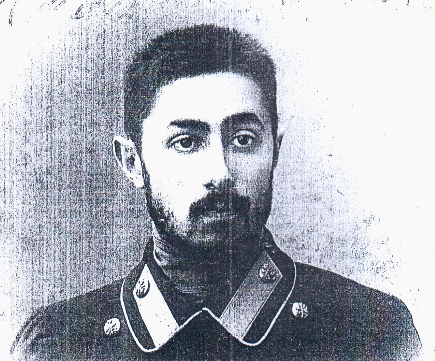
\includegraphics[scale=0.3]{figs/moses2.png} };

	\node[anchor=west] (flag) at (1.2, 1.5) { 
\includegraphics[scale=0.015]{figs/ucrania.png} };

	\node[] (dates) at (3.5, 1.5) { * \bbtext{1889} \hspace*{0.05in} \bbtext{\textdagger\ 1942} };


	\node[anchor=west] (article) at (6.0, 6.0) { \large {\bbnote{On the building blocks of mathematical logic}} };


	\node[anchor=west] (a) at (6.5, 5.0) { $\star$ \bbtext{As ideias foram apresentadas em 1920} };


	\node[anchor=west] (b) at (6.5, 4.0) { $\star$ \bbtext{O artigo foi publicado em 1924} };

\end{tikzpicture}
\end{frame}
\begin{frame}[plain,t]
\begin{tikzpicture}
\node[draw,opacity=0] at (0, 0) {x};
\node[draw,opacity=0] at (14, 8) {x};

	\node[anchor=west] (title) at (0.0, 7.0) { \Large \bbbold{Moses Schönfinkel} };

	\node[] (moses) at (3.0, 4.0) { 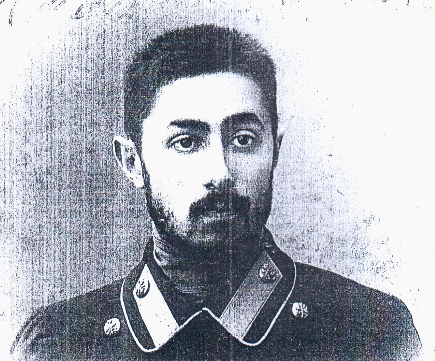
\includegraphics[scale=0.3]{figs/moses2.png} };

	\node[anchor=west] (flag) at (1.2, 1.5) { 
\includegraphics[scale=0.015]{figs/ucrania.png} };

	\node[] (dates) at (3.5, 1.5) { * \bbtext{1889} \hspace*{0.05in} \bbtext{\textdagger\ 1942} };


	\node[anchor=west] (article) at (6.0, 6.0) { \large {\bbnote{On the building blocks of mathematical logic}} };


	\node[anchor=west] (a) at (6.5, 5.0) { $\star$ \bbtext{As ideias foram apresentadas em 1920} };


	\node[anchor=west] (b) at (6.5, 4.0) { $\star$ \bbtext{O artigo foi publicado em 1924} };


	\node[anchor=west] (c) at (6.5, 3.0) { $\star$ \bbtext{Introduziu os combinadores} };

\end{tikzpicture}
\end{frame}
\begin{frame}[plain,t]
\begin{tikzpicture}
\node[draw,opacity=0] at (0, 0) {x};
\node[draw,opacity=0] at (14, 8) {x};

	\node[anchor=west] (title) at (0.0, 7.0) { \Large \bbbold{Moses Schönfinkel} };

	\node[] (moses) at (3.0, 4.0) { 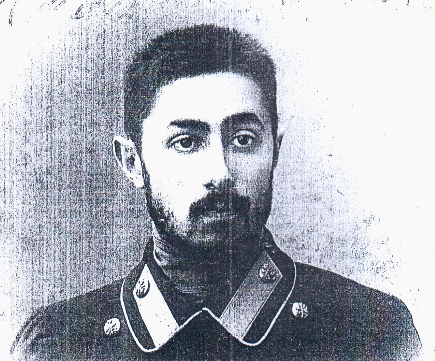
\includegraphics[scale=0.3]{figs/moses2.png} };

	\node[anchor=west] (flag) at (1.2, 1.5) { 
\includegraphics[scale=0.015]{figs/ucrania.png} };

	\node[] (dates) at (3.5, 1.5) { * \bbtext{1889} \hspace*{0.05in} \bbtext{\textdagger\ 1942} };


	\node[anchor=west] (article) at (6.0, 6.0) { \large {\bbnote{On the building blocks of mathematical logic}} };


	\node[anchor=west] (a) at (6.5, 5.0) { $\star$ \bbtext{As ideias foram apresentadas em 1920} };


	\node[anchor=west] (b) at (6.5, 4.0) { $\star$ \bbtext{O artigo foi publicado em 1924} };


	\node[anchor=west] (c) at (6.5, 3.0) { $\star$ \bbtext{Introduziu os combinadores} };


	\node[anchor=west] (d) at (6.5, 2.0) { $\star$ \bbtext{Resgatou a ideia de Frege (1893) de tratar} };

	\node[anchor=west] (d1) at (6.0, 1.4) { \bbtext{todas as funções como unárias (\bbenglish{currying})} };

\end{tikzpicture}
\end{frame}
\begin{frame}[plain,t]
\begin{tikzpicture}
\node[draw,opacity=0] at (0, 0) {x};
\node[draw,opacity=0] at (14, 8) {x};

	\node[anchor=west] (title) at (0.0, 7.0) { \Large \bbbold{Conectivos da lógica proposicional booleana} };

\end{tikzpicture}
\end{frame}
\begin{frame}[plain,t]
\begin{tikzpicture}
\node[draw,opacity=0] at (0, 0) {x};
\node[draw,opacity=0] at (14, 8) {x};

	\node[anchor=west] (title) at (0.0, 7.0) { \Large \bbbold{Conectivos da lógica proposicional booleana} };


	\draw[very thick] (0.0, 6.0) to  (13.0, 6.0);

	\draw[thick] (0.0, 5.0) to  (13.0, 5.0);

	\node[anchor=west] (op) at (0.25, 5.5) { \bbemph{Operação$^1$} };

	\node[anchor=west] (read) at (3.0, 5.5) { \bbemph{Leitura} };

	\node[anchor=west] (desc) at (5.5, 5.5) { \bbemph{Definição} };

\end{tikzpicture}
\end{frame}
\begin{frame}[plain,t]
\begin{tikzpicture}
\node[draw,opacity=0] at (0, 0) {x};
\node[draw,opacity=0] at (14, 8) {x};

	\node[anchor=west] (title) at (0.0, 7.0) { \Large \bbbold{Conectivos da lógica proposicional booleana} };


	\draw[very thick] (0.0, 6.0) to  (13.0, 6.0);

	\draw[thick] (0.0, 5.0) to  (13.0, 5.0);

	\node[anchor=west] (op) at (0.25, 5.5) { \bbemph{Operação$^1$} };

	\node[anchor=west] (read) at (3.0, 5.5) { \bbemph{Leitura} };

	\node[anchor=west] (desc) at (5.5, 5.5) { \bbemph{Definição} };


	\node[] (not) at (1.2, 4.5) { $\bar{a}$ };

	\node[] (not_read) at (3.8, 4.5) { \footnotesize \bbtext{não $a$} };

	\node[anchor=west] (not_desc) at (5.5, 4.5) { \footnotesize \bbtext{Inverte o valor lógico de $a$} };

\end{tikzpicture}
\end{frame}
\begin{frame}[plain,t]
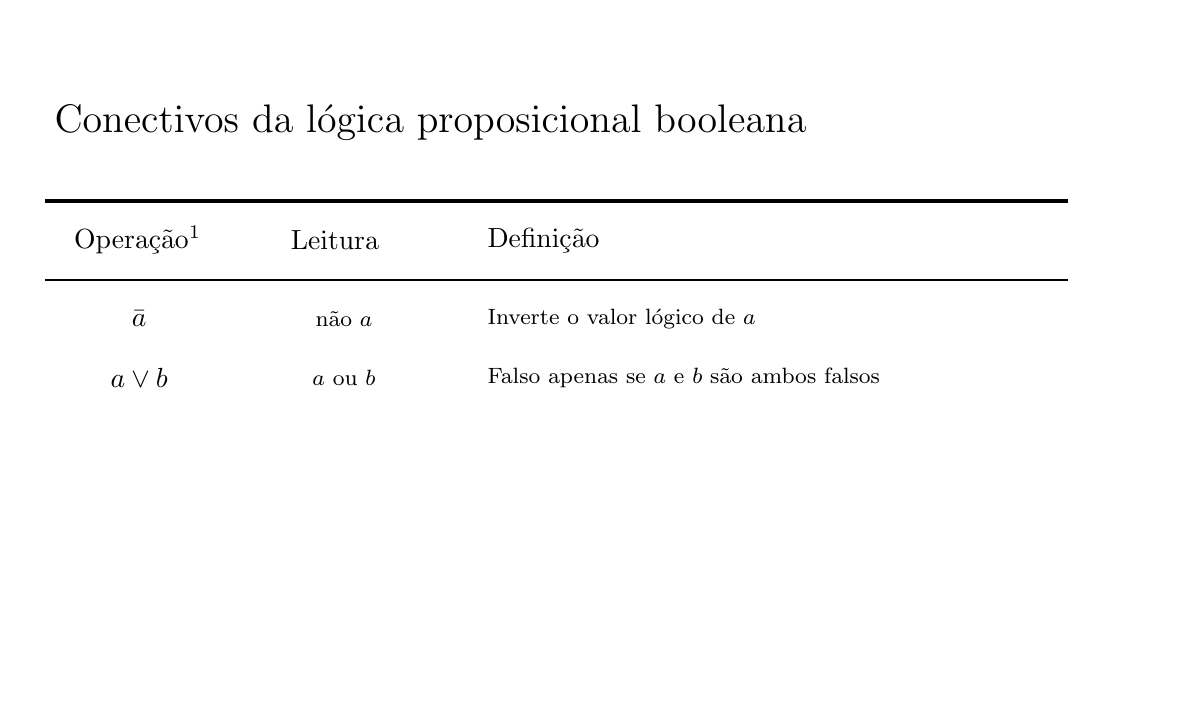
\begin{tikzpicture}
\node[draw,opacity=0] at (0, 0) {x};
\node[draw,opacity=0] at (14, 8) {x};

	\node[anchor=west] (title) at (0.0, 7.0) { \Large \bbbold{Conectivos da lógica proposicional booleana} };


	\draw[very thick] (0.0, 6.0) to  (13.0, 6.0);

	\draw[thick] (0.0, 5.0) to  (13.0, 5.0);

	\node[anchor=west] (op) at (0.25, 5.5) { \bbemph{Operação$^1$} };

	\node[anchor=west] (read) at (3.0, 5.5) { \bbemph{Leitura} };

	\node[anchor=west] (desc) at (5.5, 5.5) { \bbemph{Definição} };


	\node[] (not) at (1.2, 4.5) { $\bar{a}$ };

	\node[] (not_read) at (3.8, 4.5) { \footnotesize \bbtext{não $a$} };

	\node[anchor=west] (not_desc) at (5.5, 4.5) { \footnotesize \bbtext{Inverte o valor lógico de $a$} };


	\node[] (or) at (1.2, 3.75) { $a\vee b$ };

	\node[] (or_read) at (3.8, 3.75) { \footnotesize \bbtext{$a$ ou $b$} };

	\node[anchor=west] (or_desc) at (5.5, 3.75) { \footnotesize \bbtext{Falso apenas se $a$ e $b$ são ambos falsos} };

\end{tikzpicture}
\end{frame}
\begin{frame}[plain,t]
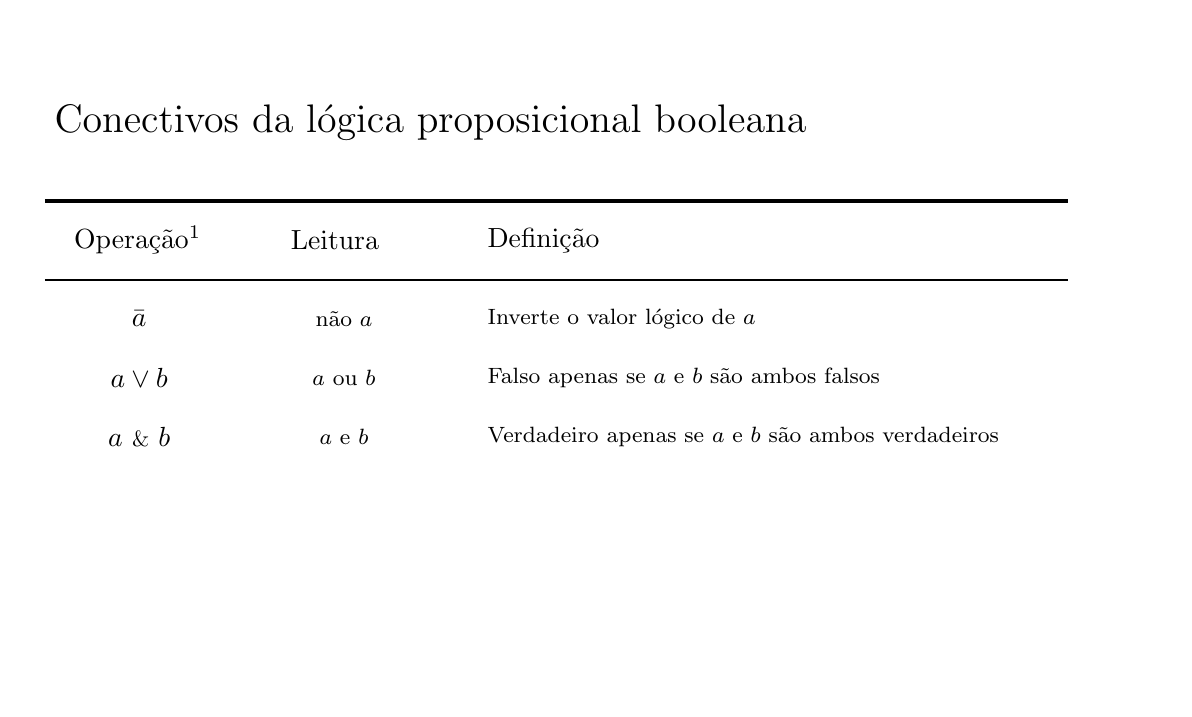
\begin{tikzpicture}
\node[draw,opacity=0] at (0, 0) {x};
\node[draw,opacity=0] at (14, 8) {x};

	\node[anchor=west] (title) at (0.0, 7.0) { \Large \bbbold{Conectivos da lógica proposicional booleana} };


	\draw[very thick] (0.0, 6.0) to  (13.0, 6.0);

	\draw[thick] (0.0, 5.0) to  (13.0, 5.0);

	\node[anchor=west] (op) at (0.25, 5.5) { \bbemph{Operação$^1$} };

	\node[anchor=west] (read) at (3.0, 5.5) { \bbemph{Leitura} };

	\node[anchor=west] (desc) at (5.5, 5.5) { \bbemph{Definição} };


	\node[] (not) at (1.2, 4.5) { $\bar{a}$ };

	\node[] (not_read) at (3.8, 4.5) { \footnotesize \bbtext{não $a$} };

	\node[anchor=west] (not_desc) at (5.5, 4.5) { \footnotesize \bbtext{Inverte o valor lógico de $a$} };


	\node[] (or) at (1.2, 3.75) { $a\vee b$ };

	\node[] (or_read) at (3.8, 3.75) { \footnotesize \bbtext{$a$ ou $b$} };

	\node[anchor=west] (or_desc) at (5.5, 3.75) { \footnotesize \bbtext{Falso apenas se $a$ e $b$ são ambos falsos} };


	\node[] (and) at (1.2, 3.0) { $a\ \scalebox{0.8}\&\  b$ };

	\node[] (and_read) at (3.8, 3.0) { \footnotesize \bbtext{$a$ e $b$} };

	\node[anchor=west] (and_desc) at (5.5, 3.0) { \footnotesize \bbtext{Verdadeiro apenas se $a$ e $b$ são ambos verdadeiros} };

\end{tikzpicture}
\end{frame}
\begin{frame}[plain,t]
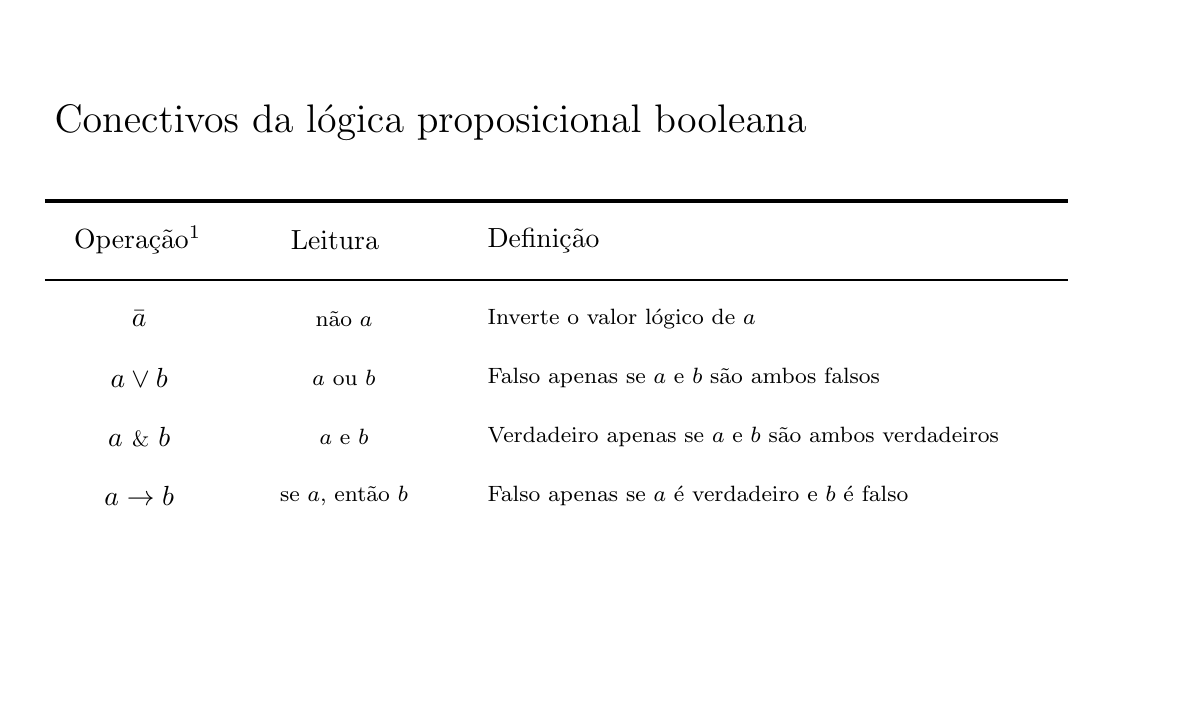
\begin{tikzpicture}
\node[draw,opacity=0] at (0, 0) {x};
\node[draw,opacity=0] at (14, 8) {x};

	\node[anchor=west] (title) at (0.0, 7.0) { \Large \bbbold{Conectivos da lógica proposicional booleana} };


	\draw[very thick] (0.0, 6.0) to  (13.0, 6.0);

	\draw[thick] (0.0, 5.0) to  (13.0, 5.0);

	\node[anchor=west] (op) at (0.25, 5.5) { \bbemph{Operação$^1$} };

	\node[anchor=west] (read) at (3.0, 5.5) { \bbemph{Leitura} };

	\node[anchor=west] (desc) at (5.5, 5.5) { \bbemph{Definição} };


	\node[] (not) at (1.2, 4.5) { $\bar{a}$ };

	\node[] (not_read) at (3.8, 4.5) { \footnotesize \bbtext{não $a$} };

	\node[anchor=west] (not_desc) at (5.5, 4.5) { \footnotesize \bbtext{Inverte o valor lógico de $a$} };


	\node[] (or) at (1.2, 3.75) { $a\vee b$ };

	\node[] (or_read) at (3.8, 3.75) { \footnotesize \bbtext{$a$ ou $b$} };

	\node[anchor=west] (or_desc) at (5.5, 3.75) { \footnotesize \bbtext{Falso apenas se $a$ e $b$ são ambos falsos} };


	\node[] (and) at (1.2, 3.0) { $a\ \scalebox{0.8}\&\  b$ };

	\node[] (and_read) at (3.8, 3.0) { \footnotesize \bbtext{$a$ e $b$} };

	\node[anchor=west] (and_desc) at (5.5, 3.0) { \footnotesize \bbtext{Verdadeiro apenas se $a$ e $b$ são ambos verdadeiros} };


	\node[] (conditional) at (1.2, 2.25) { $a \to  b$ };

	\node[] (conditional_read) at (3.8, 2.25) { \footnotesize \bbtext{se $a$, então $b$} };

	\node[anchor=west] (conditional_desc) at (5.5, 2.25) { \footnotesize \bbtext{Falso apenas se $a$ é verdadeiro e $b$ é falso} };

\end{tikzpicture}
\end{frame}
\begin{frame}[plain,t]
\begin{tikzpicture}
\node[draw,opacity=0] at (0, 0) {x};
\node[draw,opacity=0] at (14, 8) {x};

	\node[anchor=west] (title) at (0.0, 7.0) { \Large \bbbold{Conectivos da lógica proposicional booleana} };


	\draw[very thick] (0.0, 6.0) to  (13.0, 6.0);

	\draw[thick] (0.0, 5.0) to  (13.0, 5.0);

	\node[anchor=west] (op) at (0.25, 5.5) { \bbemph{Operação$^1$} };

	\node[anchor=west] (read) at (3.0, 5.5) { \bbemph{Leitura} };

	\node[anchor=west] (desc) at (5.5, 5.5) { \bbemph{Definição} };


	\node[] (not) at (1.2, 4.5) { $\bar{a}$ };

	\node[] (not_read) at (3.8, 4.5) { \footnotesize \bbtext{não $a$} };

	\node[anchor=west] (not_desc) at (5.5, 4.5) { \footnotesize \bbtext{Inverte o valor lógico de $a$} };


	\node[] (or) at (1.2, 3.75) { $a\vee b$ };

	\node[] (or_read) at (3.8, 3.75) { \footnotesize \bbtext{$a$ ou $b$} };

	\node[anchor=west] (or_desc) at (5.5, 3.75) { \footnotesize \bbtext{Falso apenas se $a$ e $b$ são ambos falsos} };


	\node[] (and) at (1.2, 3.0) { $a\ \scalebox{0.8}\&\  b$ };

	\node[] (and_read) at (3.8, 3.0) { \footnotesize \bbtext{$a$ e $b$} };

	\node[anchor=west] (and_desc) at (5.5, 3.0) { \footnotesize \bbtext{Verdadeiro apenas se $a$ e $b$ são ambos verdadeiros} };


	\node[] (conditional) at (1.2, 2.25) { $a \to  b$ };

	\node[] (conditional_read) at (3.8, 2.25) { \footnotesize \bbtext{se $a$, então $b$} };

	\node[anchor=west] (conditional_desc) at (5.5, 2.25) { \footnotesize \bbtext{Falso apenas se $a$ é verdadeiro e $b$ é falso} };


	\node[] (equivalence) at (1.2, 1.5) { $a\ \scalebox{1.2}[0.8]{\sim}\ b$ };

	\node[] (equivalence_read) at (3.8, 1.5) { \footnotesize \bbtext{$a$ é equivalente a $b$} };

	\node[anchor=west] (equivalence_desc) at (5.5, 1.5) { \footnotesize \bbtext{Verdadeiro se ambos tem mesmo valor lógico} };


	\draw[very thick] (0.0, 1.0) to  (13.0, 1.0);

\end{tikzpicture}
\end{frame}
\begin{frame}[plain,t]
\begin{tikzpicture}
\node[draw,opacity=0] at (0, 0) {x};
\node[draw,opacity=0] at (14, 8) {x};

	\node[anchor=west] (title) at (0.0, 7.0) { \Large \bbbold{Conectivos da lógica proposicional booleana} };


	\draw[very thick] (0.0, 6.0) to  (13.0, 6.0);

	\draw[thick] (0.0, 5.0) to  (13.0, 5.0);

	\node[anchor=west] (op) at (0.25, 5.5) { \bbemph{Operação$^1$} };

	\node[anchor=west] (read) at (3.0, 5.5) { \bbemph{Leitura} };

	\node[anchor=west] (desc) at (5.5, 5.5) { \bbemph{Definição} };


	\node[] (not) at (1.2, 4.5) { $\bar{a}$ };

	\node[] (not_read) at (3.8, 4.5) { \footnotesize \bbtext{não $a$} };

	\node[anchor=west] (not_desc) at (5.5, 4.5) { \footnotesize \bbtext{Inverte o valor lógico de $a$} };


	\node[] (or) at (1.2, 3.75) { $a\vee b$ };

	\node[] (or_read) at (3.8, 3.75) { \footnotesize \bbtext{$a$ ou $b$} };

	\node[anchor=west] (or_desc) at (5.5, 3.75) { \footnotesize \bbtext{Falso apenas se $a$ e $b$ são ambos falsos} };


	\node[] (and) at (1.2, 3.0) { $a\ \scalebox{0.8}\&\  b$ };

	\node[] (and_read) at (3.8, 3.0) { \footnotesize \bbtext{$a$ e $b$} };

	\node[anchor=west] (and_desc) at (5.5, 3.0) { \footnotesize \bbtext{Verdadeiro apenas se $a$ e $b$ são ambos verdadeiros} };


	\node[] (conditional) at (1.2, 2.25) { $a \to  b$ };

	\node[] (conditional_read) at (3.8, 2.25) { \footnotesize \bbtext{se $a$, então $b$} };

	\node[anchor=west] (conditional_desc) at (5.5, 2.25) { \footnotesize \bbtext{Falso apenas se $a$ é verdadeiro e $b$ é falso} };


	\node[] (equivalence) at (1.2, 1.5) { $a\ \scalebox{1.2}[0.8]{\sim}\ b$ };

	\node[] (equivalence_read) at (3.8, 1.5) { \footnotesize \bbtext{$a$ é equivalente a $b$} };

	\node[anchor=west] (equivalence_desc) at (5.5, 1.5) { \footnotesize \bbtext{Verdadeiro se ambos tem mesmo valor lógico} };


	\draw[very thick] (0.0, 1.0) to  (13.0, 1.0);


	\node[anchor=west] (footnote) at (0.5, 0.6) { \footnotesize \bbtext{$^1$\ Notação de Hilbert} };

\end{tikzpicture}
\end{frame}
\begin{frame}[plain,t]
\begin{tikzpicture}
\node[draw,opacity=0] at (0, 0) {x};
\node[draw,opacity=0] at (14, 8) {x};

	\node[anchor=west] (title) at (0.0, 7.0) { \Large \bbbold{Redução tradicional (linguagens de programação)} };

\end{tikzpicture}
\end{frame}
\begin{frame}[plain,t]
\begin{tikzpicture}
\node[draw,opacity=0] at (0, 0) {x};
\node[draw,opacity=0] at (14, 8) {x};

	\node[anchor=west] (title) at (0.0, 7.0) { \Large \bbbold{Redução tradicional (linguagens de programação)} };


	\node[anchor=west] (label) at (1.0, 5.0) { \large \bbbold{Primitivos:}\ \ {\large $\bar{}, \scalebox{0.7}{\&}, \vee$} };

\end{tikzpicture}
\end{frame}
\begin{frame}[plain,t]
\begin{tikzpicture}
\node[draw,opacity=0] at (0, 0) {x};
\node[draw,opacity=0] at (14, 8) {x};

	\node[anchor=west] (title) at (0.0, 7.0) { \Large \bbbold{Redução tradicional (linguagens de programação)} };


	\node[anchor=west] (label) at (1.0, 5.0) { \large \bbbold{Primitivos:}\ \ {\large $\bar{}, \scalebox{0.7}{\&}, \vee$} };


	\node[anchor=west] (label2) at (1.0, 4.0) { \large \bbbold{Reduções:} };

\end{tikzpicture}
\end{frame}
\begin{frame}[plain,t]
\begin{tikzpicture}
\node[draw,opacity=0] at (0, 0) {x};
\node[draw,opacity=0] at (14, 8) {x};

	\node[anchor=west] (title) at (0.0, 7.0) { \Large \bbbold{Redução tradicional (linguagens de programação)} };


	\node[anchor=west] (label) at (1.0, 5.0) { \large \bbbold{Primitivos:}\ \ {\large $\bar{}, \scalebox{0.7}{\&}, \vee$} };


	\node[anchor=west] (label2) at (1.0, 4.0) { \large \bbbold{Reduções:} };


	\node[] (conditional) at (7.0, 3.5) { \Large $p \to q\ \equiv \ \bar{p}\vee q$ };

\end{tikzpicture}
\end{frame}
\begin{frame}[plain,t]
\begin{tikzpicture}
\node[draw,opacity=0] at (0, 0) {x};
\node[draw,opacity=0] at (14, 8) {x};

	\node[anchor=west] (title) at (0.0, 7.0) { \Large \bbbold{Redução tradicional (linguagens de programação)} };


	\node[anchor=west] (label) at (1.0, 5.0) { \large \bbbold{Primitivos:}\ \ {\large $\bar{}, \scalebox{0.7}{\&}, \vee$} };


	\node[anchor=west] (label2) at (1.0, 4.0) { \large \bbbold{Reduções:} };


	\node[] (conditional) at (7.0, 3.5) { \Large $p \to q\ \equiv \ \bar{p}\vee q$ };


	\node[] (biconditional) at (7.0, 2.25) { \Large $p\ \scalebox{1.2}[0.8]{\sim}\ q\ \equiv\ (p\ \scalebox{0.7}{\&}\ q)\vee (\bar{p}\ \scalebox{0.7}{\&}\  \bar{q})$ };


\end{tikzpicture}
\end{frame}
\begin{frame}[plain,t]
\begin{tikzpicture}
\node[draw,opacity=0] at (0, 0) {x};
\node[draw,opacity=0] at (14, 8) {x};

	\node[anchor=west] (title) at (0.0, 7.0) { \Large \bbbold{Redução de Whitehead e Russell} };

\end{tikzpicture}
\end{frame}
\begin{frame}[plain,t]
\begin{tikzpicture}
\node[draw,opacity=0] at (0, 0) {x};
\node[draw,opacity=0] at (14, 8) {x};

	\node[anchor=west] (title) at (0.0, 7.0) { \Large \bbbold{Redução de Whitehead e Russell} };


	\node[anchor=west] (label) at (1.0, 5.0) { \large \bbbold{Primitivos:}\ \ {\large $\bar{}, \vee$} };

\end{tikzpicture}
\end{frame}
\begin{frame}[plain,t]
\begin{tikzpicture}
\node[draw,opacity=0] at (0, 0) {x};
\node[draw,opacity=0] at (14, 8) {x};

	\node[anchor=west] (title) at (0.0, 7.0) { \Large \bbbold{Redução de Whitehead e Russell} };


	\node[anchor=west] (label) at (1.0, 5.0) { \large \bbbold{Primitivos:}\ \ {\large $\bar{}, \vee$} };


	\node[anchor=west] (label2) at (1.0, 4.0) { \large \bbbold{Reduções:} };

\end{tikzpicture}
\end{frame}
\begin{frame}[plain,t]
\begin{tikzpicture}
\node[draw,opacity=0] at (0, 0) {x};
\node[draw,opacity=0] at (14, 8) {x};

	\node[anchor=west] (title) at (0.0, 7.0) { \Large \bbbold{Redução de Whitehead e Russell} };


	\node[anchor=west] (label) at (1.0, 5.0) { \large \bbbold{Primitivos:}\ \ {\large $\bar{}, \vee$} };


	\node[anchor=west] (label2) at (1.0, 4.0) { \large \bbbold{Reduções:} };

	\node[] (and) at (7.0, 3.5) { \Large $p\ \scalebox{0.8}{\&}\ q\ \equiv \overline{(\bar{p}\vee \bar{q})}$ };
\end{tikzpicture}
\end{frame}
\begin{frame}[plain,t]
\begin{tikzpicture}
\node[draw,opacity=0] at (0, 0) {x};
\node[draw,opacity=0] at (14, 8) {x};

	\node[anchor=west] (title) at (0.0, 7.0) { \Large \bbbold{Redução de Whitehead e Russell} };


	\node[anchor=west] (label) at (1.0, 5.0) { \large \bbbold{Primitivos:}\ \ {\large $\bar{}, \vee$} };


	\node[anchor=west] (label2) at (1.0, 4.0) { \large \bbbold{Reduções:} };

	\node[] (and) at (7.0, 3.5) { \Large $p\ \scalebox{0.8}{\&}\ q\ \equiv \overline{(\bar{p}\vee \bar{q})}$ };

	\node[] (conditional) at (7.0, 2.25) { \Large $p \to q\ \equiv \ \bar{p}\vee q$ };

\end{tikzpicture}
\end{frame}
\begin{frame}[plain,t]
\begin{tikzpicture}
\node[draw,opacity=0] at (0, 0) {x};
\node[draw,opacity=0] at (14, 8) {x};

	\node[anchor=west] (title) at (0.0, 7.0) { \Large \bbbold{Redução de Whitehead e Russell} };


	\node[anchor=west] (label) at (1.0, 5.0) { \large \bbbold{Primitivos:}\ \ {\large $\bar{}, \vee$} };


	\node[anchor=west] (label2) at (1.0, 4.0) { \large \bbbold{Reduções:} };

	\node[] (and) at (7.0, 3.5) { \Large $p\ \scalebox{0.8}{\&}\ q\ \equiv \overline{(\bar{p}\vee \bar{q})}$ };

	\node[] (conditional) at (7.0, 2.25) { \Large $p \to q\ \equiv \ \bar{p}\vee q$ };


	\node[] (biconditional) at (7.0, 1.0) { \Large $p\ \scalebox{1.2}[0.8]{\sim}\ q\ \equiv\ (p\to q)\ \scalebox{0.7}{\&}\ (\bar{q}\to  \bar{p})$ };

\end{tikzpicture}
\end{frame}
\begin{frame}[plain,t]
\begin{tikzpicture}
\node[draw,opacity=0] at (0, 0) {x};
\node[draw,opacity=0] at (14, 8) {x};

	\node[anchor=west] (title) at (0.0, 7.0) { \Large \bbbold{Conectivos de Scheffer} };

\end{tikzpicture}
\end{frame}
\begin{frame}[plain,t]
\begin{tikzpicture}
\node[draw,opacity=0] at (0, 0) {x};
\node[draw,opacity=0] at (14, 8) {x};

	\node[anchor=west] (title) at (0.0, 7.0) { \Large \bbbold{Conectivos de Scheffer} };


	\draw[very thick] (0.0, 6.0) to  (13.0, 6.0);

	\draw[thick] (0.0, 5.0) to  (13.0, 5.0);

	\node[anchor=west] (op) at (0.25, 5.5) { \bbemph{Conectivo} };

	\node[anchor=west] (read) at (3.0, 5.5) { \bbemph{Nome} };

	\node[anchor=west] (desc) at (5.5, 5.5) { \bbemph{Definição} };

\end{tikzpicture}
\end{frame}
\begin{frame}[plain,t]
\begin{tikzpicture}
\node[draw,opacity=0] at (0, 0) {x};
\node[draw,opacity=0] at (14, 8) {x};

	\node[anchor=west] (title) at (0.0, 7.0) { \Large \bbbold{Conectivos de Scheffer} };


	\draw[very thick] (0.0, 6.0) to  (13.0, 6.0);

	\draw[thick] (0.0, 5.0) to  (13.0, 5.0);

	\node[anchor=west] (op) at (0.25, 5.5) { \bbemph{Conectivo} };

	\node[anchor=west] (read) at (3.0, 5.5) { \bbemph{Nome} };

	\node[anchor=west] (desc) at (5.5, 5.5) { \bbemph{Definição} };


	\node[] (and) at (1.2, 4.25) { $\downarrow$ };

	\node[] (and_read) at (3.8, 4.25) { \footnotesize \bbtext{negação conjunta} };

	\node[anchor=west] (and_desc) at (5.5, 4.5) { \footnotesize \bbtext{Verdadeira somente quando ambas proposições são falsas} };

	\node[anchor=west] (and_desc2) at (5.5, 4.0) { \footnotesize $(p\downarrow q\equiv \bar{p}\ \scalebox{0.8}{\&}\ \bar{q})$ };

\end{tikzpicture}
\end{frame}
\begin{frame}[plain,t]
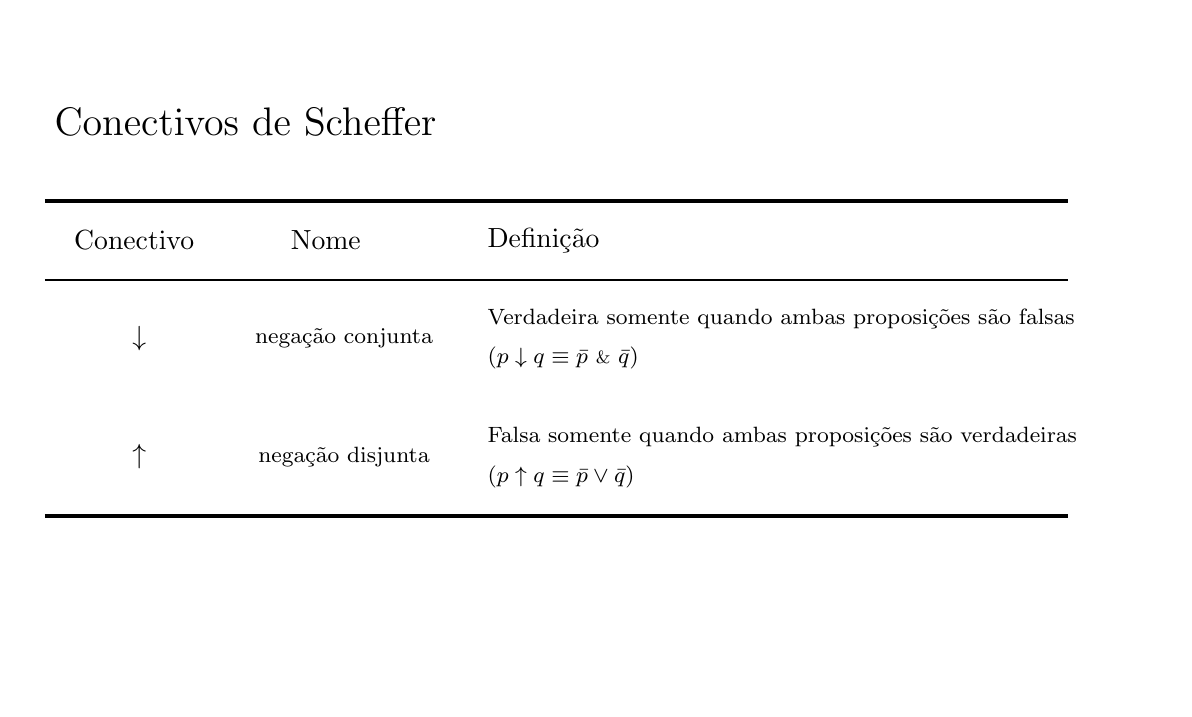
\begin{tikzpicture}
\node[draw,opacity=0] at (0, 0) {x};
\node[draw,opacity=0] at (14, 8) {x};

	\node[anchor=west] (title) at (0.0, 7.0) { \Large \bbbold{Conectivos de Scheffer} };


	\draw[very thick] (0.0, 6.0) to  (13.0, 6.0);

	\draw[thick] (0.0, 5.0) to  (13.0, 5.0);

	\node[anchor=west] (op) at (0.25, 5.5) { \bbemph{Conectivo} };

	\node[anchor=west] (read) at (3.0, 5.5) { \bbemph{Nome} };

	\node[anchor=west] (desc) at (5.5, 5.5) { \bbemph{Definição} };


	\node[] (and) at (1.2, 4.25) { $\downarrow$ };

	\node[] (and_read) at (3.8, 4.25) { \footnotesize \bbtext{negação conjunta} };

	\node[anchor=west] (and_desc) at (5.5, 4.5) { \footnotesize \bbtext{Verdadeira somente quando ambas proposições são falsas} };

	\node[anchor=west] (and_desc2) at (5.5, 4.0) { \footnotesize $(p\downarrow q\equiv \bar{p}\ \scalebox{0.8}{\&}\ \bar{q})$ };


	\node[] (not) at (1.2, 2.75) { $\uparrow$ };

	\node[] (not_read) at (3.8, 2.75) { \footnotesize \bbtext{negação disjunta} };

	\node[anchor=west] (not_desc) at (5.5, 3.0) { \footnotesize \bbtext{Falsa somente quando ambas proposições são verdadeiras} };

	\node[anchor=west] (not_desc2) at (5.5, 2.5) { \footnotesize $(p\uparrow q\equiv \bar{p}\vee \bar{q})$ };

	\draw[very thick] (0.0, 2.0) to  (13.0, 2.0);

\end{tikzpicture}
\end{frame}
\begin{frame}[plain,t]
\begin{tikzpicture}
\node[draw,opacity=0] at (0, 0) {x};
\node[draw,opacity=0] at (14, 8) {x};

	\node[anchor=west] (title) at (0.0, 7.0) { \Large \bbbold{Redução de Scheffer (1913)} };

\end{tikzpicture}
\end{frame}
\begin{frame}[plain,t]
\begin{tikzpicture}
\node[draw,opacity=0] at (0, 0) {x};
\node[draw,opacity=0] at (14, 8) {x};

	\node[anchor=west] (title) at (0.0, 7.0) { \Large \bbbold{Redução de Scheffer (1913)} };


	\node[anchor=west] (label) at (1.0, 5.0) { \large \bbbold{Primitivo:}\ \ {\large $\uparrow$} \bbtext{(notação de Schönfinkel: $p\ |\ q$)} };

\end{tikzpicture}
\end{frame}
\begin{frame}[plain,t]
\begin{tikzpicture}
\node[draw,opacity=0] at (0, 0) {x};
\node[draw,opacity=0] at (14, 8) {x};

	\node[anchor=west] (title) at (0.0, 7.0) { \Large \bbbold{Redução de Scheffer (1913)} };


	\node[anchor=west] (label) at (1.0, 5.0) { \large \bbbold{Primitivo:}\ \ {\large $\uparrow$} \bbtext{(notação de Schönfinkel: $p\ |\ q$)} };


	\node[anchor=west] (label2) at (1.0, 4.0) { \large \bbbold{Reduções:} };

\end{tikzpicture}
\end{frame}
\begin{frame}[plain,t]
\begin{tikzpicture}
\node[draw,opacity=0] at (0, 0) {x};
\node[draw,opacity=0] at (14, 8) {x};

	\node[anchor=west] (title) at (0.0, 7.0) { \Large \bbbold{Redução de Scheffer (1913)} };


	\node[anchor=west] (label) at (1.0, 5.0) { \large \bbbold{Primitivo:}\ \ {\large $\uparrow$} \bbtext{(notação de Schönfinkel: $p\ |\ q$)} };


	\node[anchor=west] (label2) at (1.0, 4.0) { \large \bbbold{Reduções:} };

	\node[] (and) at (7.0, 3.5) { \Large $p\ \scalebox{0.8}{\&}\ q\ \equiv\ (p\ |\ q)\ |\ (p\ |\ q)$ };

\end{tikzpicture}
\end{frame}
\begin{frame}[plain,t]
\begin{tikzpicture}
\node[draw,opacity=0] at (0, 0) {x};
\node[draw,opacity=0] at (14, 8) {x};

	\node[anchor=west] (title) at (0.0, 7.0) { \Large \bbbold{Redução de Scheffer (1913)} };


	\node[anchor=west] (label) at (1.0, 5.0) { \large \bbbold{Primitivo:}\ \ {\large $\uparrow$} \bbtext{(notação de Schönfinkel: $p\ |\ q$)} };


	\node[anchor=west] (label2) at (1.0, 4.0) { \large \bbbold{Reduções:} };

	\node[] (and) at (7.0, 3.5) { \Large $p\ \scalebox{0.8}{\&}\ q\ \equiv\ (p\ |\ q)\ |\ (p\ |\ q)$ };


	\node[] (or) at (7.0, 2.25) { \Large $p \vee q\ \equiv \ (p\ |\ p)\ |\ (q\ |\ q)$ };

\end{tikzpicture}
\end{frame}
\begin{frame}[plain,t]
\begin{tikzpicture}
\node[draw,opacity=0] at (0, 0) {x};
\node[draw,opacity=0] at (14, 8) {x};

	\node[anchor=west] (title) at (0.0, 7.0) { \Large \bbbold{Redução de Scheffer (1913)} };


	\node[anchor=west] (label) at (1.0, 5.0) { \large \bbbold{Primitivo:}\ \ {\large $\uparrow$} \bbtext{(notação de Schönfinkel: $p\ |\ q$)} };


	\node[anchor=west] (label2) at (1.0, 4.0) { \large \bbbold{Reduções:} };

	\node[] (and) at (7.0, 3.5) { \Large $p\ \scalebox{0.8}{\&}\ q\ \equiv\ (p\ |\ q)\ |\ (p\ |\ q)$ };


	\node[] (or) at (7.0, 2.25) { \Large $p \vee q\ \equiv \ (p\ |\ p)\ |\ (q\ |\ q)$ };


	\node[] (not) at (7.0, 1.0) { \Large $\bar{p} \equiv\ (p\ |\ p)$ };

\end{tikzpicture}
\end{frame}
\begin{frame}[plain,t]
\begin{tikzpicture}
\node[draw,opacity=0] at (0, 0) {x};
\node[draw,opacity=0] at (14, 8) {x};

	\node[anchor=west] (title) at (0.0, 7.0) { \Large \bbbold{Quantificadores} };

\end{tikzpicture}
\end{frame}
\begin{frame}[plain,t]
\begin{tikzpicture}
\node[draw,opacity=0] at (0, 0) {x};
\node[draw,opacity=0] at (14, 8) {x};

	\node[anchor=west] (title) at (0.0, 7.0) { \Large \bbbold{Quantificadores} };


	\draw[very thick] (0.0, 6.0) to  (13.0, 6.0);

	\draw[thick] (0.0, 5.0) to  (13.0, 5.0);

	\node[anchor=west] (op) at (0.25, 5.5) { \bbemph{Notação} };

	\node[anchor=west] (read) at (3.0, 5.5) { \bbemph{Nome} };

	\node[anchor=west] (desc) at (5.5, 5.5) { \bbemph{Definição} };

\end{tikzpicture}
\end{frame}
\begin{frame}[plain,t]
\begin{tikzpicture}
\node[draw,opacity=0] at (0, 0) {x};
\node[draw,opacity=0] at (14, 8) {x};

	\node[anchor=west] (title) at (0.0, 7.0) { \Large \bbbold{Quantificadores} };


	\draw[very thick] (0.0, 6.0) to  (13.0, 6.0);

	\draw[thick] (0.0, 5.0) to  (13.0, 5.0);

	\node[anchor=west] (op) at (0.25, 5.5) { \bbemph{Notação} };

	\node[anchor=west] (read) at (3.0, 5.5) { \bbemph{Nome} };

	\node[anchor=west] (desc) at (5.5, 5.5) { \bbemph{Definição} };


	\node[] (exists) at (1.2, 4.5) { $(Ex)f(x)$ };

	\node[] (exists2) at (1.2, 4.0) { $\exists x.f(x)$ };


	\node[] (exists_read) at (3.8, 4.5) { \footnotesize \bbtext{quantificador} };

	\node[] (exists_read2) at (3.8, 4.0) { \footnotesize \bbtext{existencial} };


	\node[anchor=west] (exists_desc) at (5.5, 4.25) { \footnotesize \bbtext{Existe ao menos um $x$ que tem a propriedade $f$} };

\end{tikzpicture}
\end{frame}
\begin{frame}[plain,t]
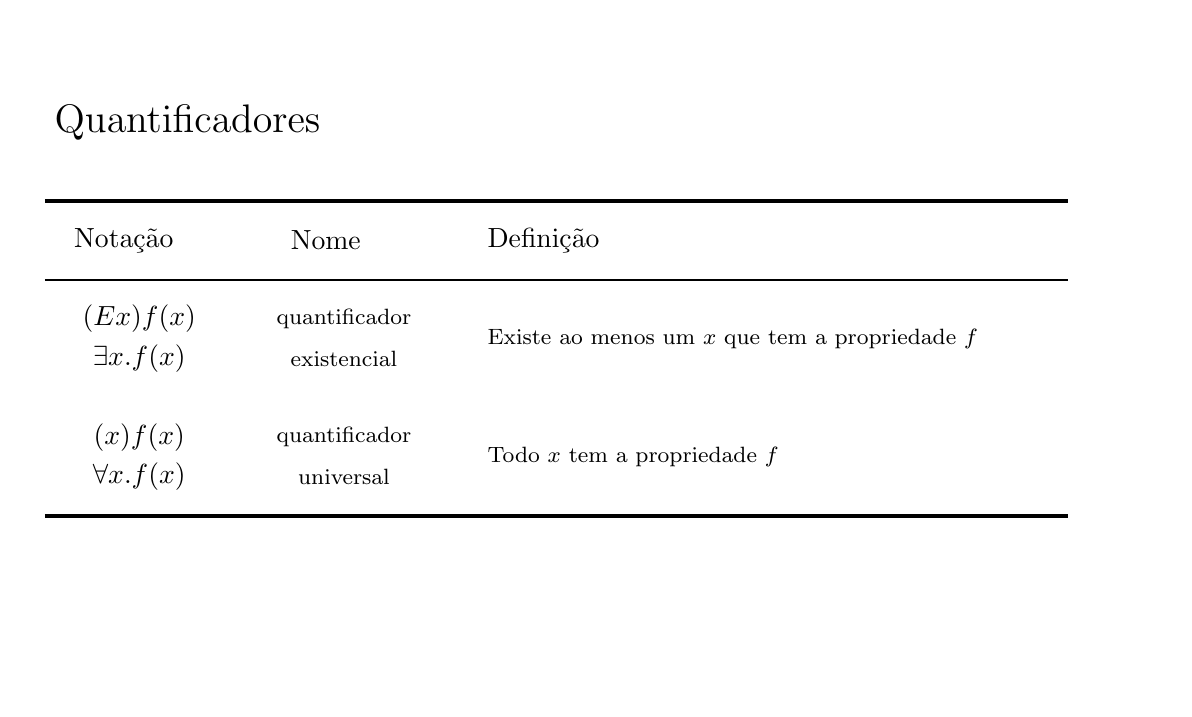
\begin{tikzpicture}
\node[draw,opacity=0] at (0, 0) {x};
\node[draw,opacity=0] at (14, 8) {x};

	\node[anchor=west] (title) at (0.0, 7.0) { \Large \bbbold{Quantificadores} };


	\draw[very thick] (0.0, 6.0) to  (13.0, 6.0);

	\draw[thick] (0.0, 5.0) to  (13.0, 5.0);

	\node[anchor=west] (op) at (0.25, 5.5) { \bbemph{Notação} };

	\node[anchor=west] (read) at (3.0, 5.5) { \bbemph{Nome} };

	\node[anchor=west] (desc) at (5.5, 5.5) { \bbemph{Definição} };


	\node[] (exists) at (1.2, 4.5) { $(Ex)f(x)$ };

	\node[] (exists2) at (1.2, 4.0) { $\exists x.f(x)$ };


	\node[] (exists_read) at (3.8, 4.5) { \footnotesize \bbtext{quantificador} };

	\node[] (exists_read2) at (3.8, 4.0) { \footnotesize \bbtext{existencial} };


	\node[anchor=west] (exists_desc) at (5.5, 4.25) { \footnotesize \bbtext{Existe ao menos um $x$ que tem a propriedade $f$} };


	\node[] (forall) at (1.2, 3.0) { $(x)f(x)$ };

	\node[] (forall2) at (1.2, 2.5) { $\forall x.f(x)$ };


	\node[] (forall_read) at (3.8, 3.0) { \footnotesize \bbtext{quantificador} };

	\node[] (forall_read2) at (3.8, 2.5) { \footnotesize \bbtext{universal} };


	\node[anchor=west] (forall_desc) at (5.5, 2.75) { \footnotesize \bbtext{Todo $x$ tem a propriedade $f$} };

	\draw[very thick] (0.0, 2.0) to  (13.0, 2.0);

\end{tikzpicture}
\end{frame}
\begin{frame}[plain,t]
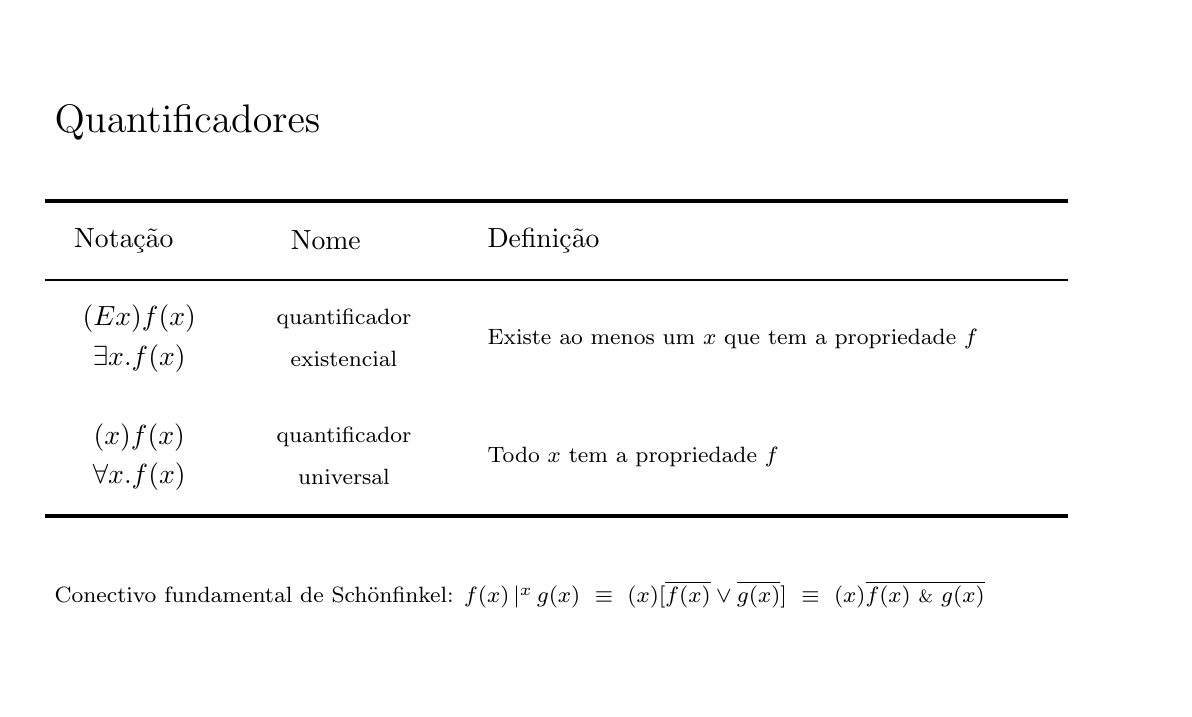
\begin{tikzpicture}
\node[draw,opacity=0] at (0, 0) {x};
\node[draw,opacity=0] at (14, 8) {x};

	\node[anchor=west] (title) at (0.0, 7.0) { \Large \bbbold{Quantificadores} };


	\draw[very thick] (0.0, 6.0) to  (13.0, 6.0);

	\draw[thick] (0.0, 5.0) to  (13.0, 5.0);

	\node[anchor=west] (op) at (0.25, 5.5) { \bbemph{Notação} };

	\node[anchor=west] (read) at (3.0, 5.5) { \bbemph{Nome} };

	\node[anchor=west] (desc) at (5.5, 5.5) { \bbemph{Definição} };


	\node[] (exists) at (1.2, 4.5) { $(Ex)f(x)$ };

	\node[] (exists2) at (1.2, 4.0) { $\exists x.f(x)$ };


	\node[] (exists_read) at (3.8, 4.5) { \footnotesize \bbtext{quantificador} };

	\node[] (exists_read2) at (3.8, 4.0) { \footnotesize \bbtext{existencial} };


	\node[anchor=west] (exists_desc) at (5.5, 4.25) { \footnotesize \bbtext{Existe ao menos um $x$ que tem a propriedade $f$} };


	\node[] (forall) at (1.2, 3.0) { $(x)f(x)$ };

	\node[] (forall2) at (1.2, 2.5) { $\forall x.f(x)$ };


	\node[] (forall_read) at (3.8, 3.0) { \footnotesize \bbtext{quantificador} };

	\node[] (forall_read2) at (3.8, 2.5) { \footnotesize \bbtext{universal} };


	\node[anchor=west] (forall_desc) at (5.5, 2.75) { \footnotesize \bbtext{Todo $x$ tem a propriedade $f$} };

	\draw[very thick] (0.0, 2.0) to  (13.0, 2.0);


	\node[anchor=west] (connective) at (0.0, 1.0) { \footnotesize \bbbold{Conectivo fundamental de Schönfinkel}: $f(x)\, |^x\, g(x)\ \equiv\ (x)[\overline{f(x)}\vee\overline{g(x)}]\ \equiv\ (x)\overline{f(x)\ \scalebox{0.8}{\&}\ g(x)}$ };

\end{tikzpicture}
\end{frame}
\begin{frame}[plain,t]
\begin{tikzpicture}
\node[draw,opacity=0] at (0, 0) {x};
\node[draw,opacity=0] at (14, 8) {x};

	\node[anchor=west] (title) at (0.0, 7.0) { \Large \bbbold{Reduções de Schönfinkel} };

\end{tikzpicture}
\end{frame}
\begin{frame}[plain,t]
\begin{tikzpicture}
\node[draw,opacity=0] at (0, 0) {x};
\node[draw,opacity=0] at (14, 8) {x};

	\node[anchor=west] (title) at (0.0, 7.0) { \Large \bbbold{Reduções de Schönfinkel} };


	\node[anchor=west] (label) at (0.0, 6.0) { \large \bbbold{Primitivo:}\ \ {\large $f(x)\, |^x\,  g(x)$} };

\end{tikzpicture}
\end{frame}
\begin{frame}[plain,t]
\begin{tikzpicture}
\node[draw,opacity=0] at (0, 0) {x};
\node[draw,opacity=0] at (14, 8) {x};

	\node[anchor=west] (title) at (0.0, 7.0) { \Large \bbbold{Reduções de Schönfinkel} };


	\node[anchor=west] (label) at (0.0, 6.0) { \large \bbbold{Primitivo:}\ \ {\large $f(x)\, |^x\,  g(x)$} };


	\node[anchor=west] (label2) at (0.0, 5.0) { \large \bbbold{Reduções:} };

\end{tikzpicture}
\end{frame}
\begin{frame}[plain,t]
\begin{tikzpicture}
\node[draw,opacity=0] at (0, 0) {x};
\node[draw,opacity=0] at (14, 8) {x};

	\node[anchor=west] (title) at (0.0, 7.0) { \Large \bbbold{Reduções de Schönfinkel} };


	\node[anchor=west] (label) at (0.0, 6.0) { \large \bbbold{Primitivo:}\ \ {\large $f(x)\, |^x\,  g(x)$} };


	\node[anchor=west] (label2) at (0.0, 5.0) { \large \bbbold{Reduções:} };


	\node[anchor=west] (not) at (0.5, 4.0) { \large $\bar{a} = a\, |^x\,  a$ };

\end{tikzpicture}
\end{frame}
\begin{frame}[plain,t]
\begin{tikzpicture}
\node[draw,opacity=0] at (0, 0) {x};
\node[draw,opacity=0] at (14, 8) {x};

	\node[anchor=west] (title) at (0.0, 7.0) { \Large \bbbold{Reduções de Schönfinkel} };


	\node[anchor=west] (label) at (0.0, 6.0) { \large \bbbold{Primitivo:}\ \ {\large $f(x)\, |^x\,  g(x)$} };


	\node[anchor=west] (label2) at (0.0, 5.0) { \large \bbbold{Reduções:} };


	\node[anchor=west] (not) at (0.5, 4.0) { \large $\bar{a} = a\, |^x\,  a$ };


	\node[anchor=west] (or) at (0.5, 3.0) { \large $a\vee b = (x)(a\vee b) = \bar{a}\, |^x\,  \bar{b} = (a\, |^y\,  a)\, |^x\,  (b\, |^y\, b)$ };

\end{tikzpicture}
\end{frame}
\begin{frame}[plain,t]
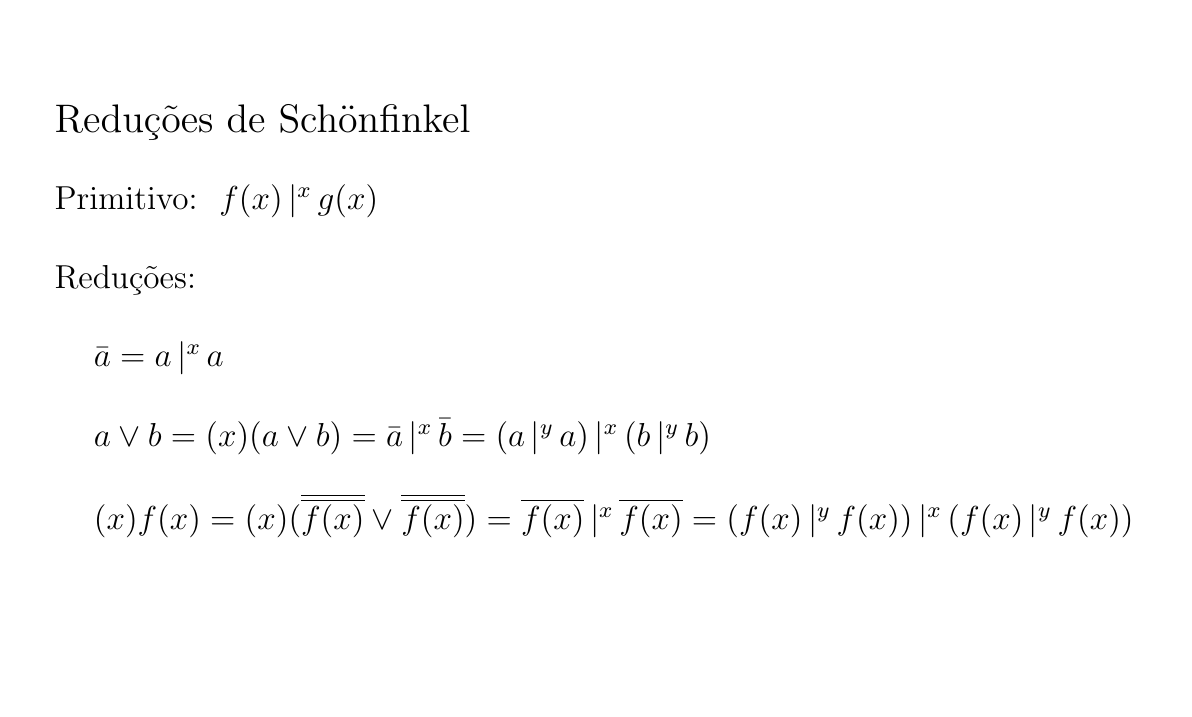
\begin{tikzpicture}
\node[draw,opacity=0] at (0, 0) {x};
\node[draw,opacity=0] at (14, 8) {x};

	\node[anchor=west] (title) at (0.0, 7.0) { \Large \bbbold{Reduções de Schönfinkel} };


	\node[anchor=west] (label) at (0.0, 6.0) { \large \bbbold{Primitivo:}\ \ {\large $f(x)\, |^x\,  g(x)$} };


	\node[anchor=west] (label2) at (0.0, 5.0) { \large \bbbold{Reduções:} };


	\node[anchor=west] (not) at (0.5, 4.0) { \large $\bar{a} = a\, |^x\,  a$ };


	\node[anchor=west] (or) at (0.5, 3.0) { \large $a\vee b = (x)(a\vee b) = \bar{a}\, |^x\,  \bar{b} = (a\, |^y\,  a)\, |^x\,  (b\, |^y\, b)$ };


	\node[anchor=west] (exists) at (0.5, 2.0) { \large $(x)f(x) = (x)(\overline{\overline{f(x)}}\vee \overline{\overline{f(x)}})  = \overline{f(x)}\, |^x\, \overline{f(x)} = (f(x)\, |^y\, f(x))\, |^x\, (f(x)\, |^y\, f(x))$ };

\end{tikzpicture}
\end{frame}
\begin{frame}[plain,t]
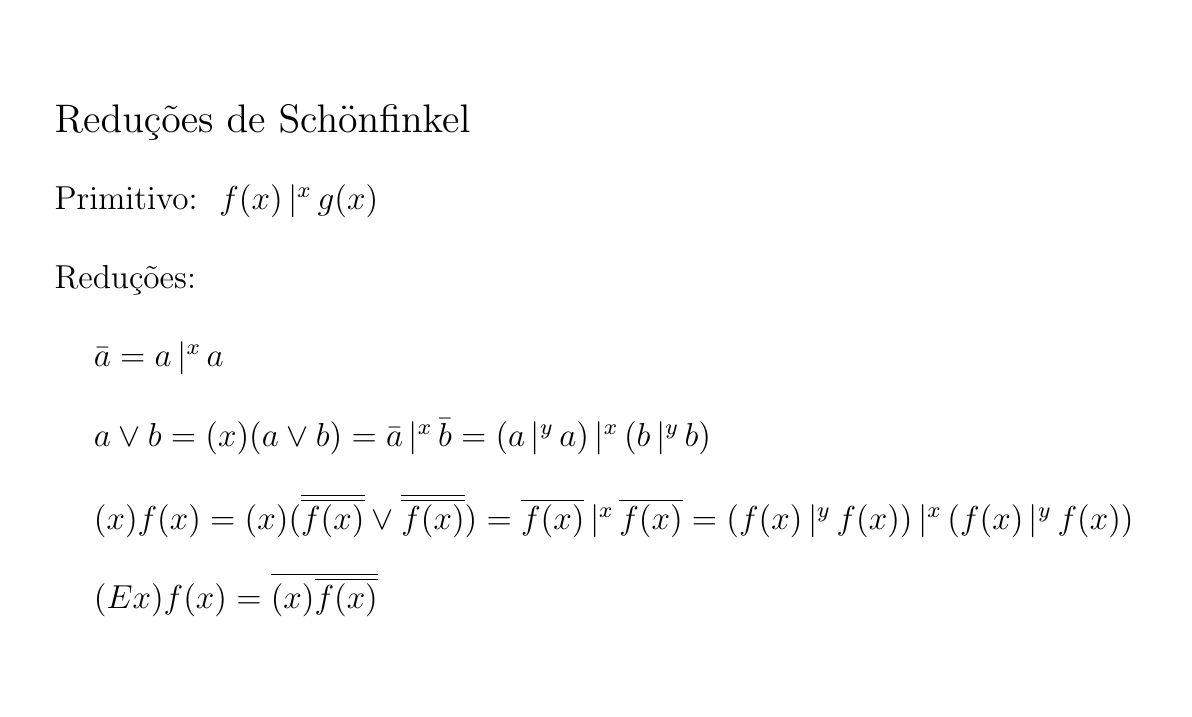
\begin{tikzpicture}
\node[draw,opacity=0] at (0, 0) {x};
\node[draw,opacity=0] at (14, 8) {x};

	\node[anchor=west] (title) at (0.0, 7.0) { \Large \bbbold{Reduções de Schönfinkel} };


	\node[anchor=west] (label) at (0.0, 6.0) { \large \bbbold{Primitivo:}\ \ {\large $f(x)\, |^x\,  g(x)$} };


	\node[anchor=west] (label2) at (0.0, 5.0) { \large \bbbold{Reduções:} };


	\node[anchor=west] (not) at (0.5, 4.0) { \large $\bar{a} = a\, |^x\,  a$ };


	\node[anchor=west] (or) at (0.5, 3.0) { \large $a\vee b = (x)(a\vee b) = \bar{a}\, |^x\,  \bar{b} = (a\, |^y\,  a)\, |^x\,  (b\, |^y\, b)$ };


	\node[anchor=west] (exists) at (0.5, 2.0) { \large $(x)f(x) = (x)(\overline{\overline{f(x)}}\vee \overline{\overline{f(x)}})  = \overline{f(x)}\, |^x\, \overline{f(x)} = (f(x)\, |^y\, f(x))\, |^x\, (f(x)\, |^y\, f(x))$ };


	\node[anchor=west] (forall) at (0.5, 1.0) { \large $(Ex)f(x) = \overline{(x)\overline{f(x)}}$ };

\end{tikzpicture}
\end{frame}
\begin{frame}[plain,t]
\vspace*{\fill}

\begin{tikzpicture}
\node[draw,opacity=0] at (0, 0) {x};
\node[draw,opacity=0] at (14, 8) {x};
\node[anchor=west] (title) at (0.0, 7.0) { \Large \bbbold{Cálculo funcional} };

\node[anchor=west] at (0, 3.5) {\begin{tcolorbox}[colback=blue!5,colframe=blue!60!green,title=\textbf{Funções de um argumento}]
\bbtext{Uma função $f$ de um argumento $x$ pode ser representada pela justaposição dos símbolos da função e de seu argumento. Em notação matemática,}
$$
f(x)\ \equiv\ fx
$$
\end{tcolorbox}};

\end{tikzpicture}

\vspace*{\fill}
\end{frame}
\begin{frame}[plain,t]
\vspace*{\fill}

\begin{tikzpicture}
\node[draw,opacity=0] at (0, 0) {x};
\node[draw,opacity=0] at (14, 8) {x};
\node[anchor=west] (title) at (0.0, 7.5) { \Large \bbbold{Cálculo funcional} };

\node[anchor=west] at (0, 3.5) {\begin{tcolorbox}[colback=blue!5,colframe=blue!60!green,title=\textbf{Funções de vários argumentos}]
\bbtext{Uma função $F(x, y)$ de dois argumentos pode ser reduzida a duas funções de um único argumento. Defina, para um $x$ fixo, a função
$G_x(y)$ tal que $G_x(y) = F(x, y)$. Ou seja, uma vez fixado $x$, $G_x$ coincide com $F$ em todos os pares $(x, y)$. Como $G$ é uma função de um
único argumento, podemos escrever $G = fx$ e}
$$
F(x, y) = G_x(y) = (G_x)y = (fx)y = fxy
$$
\bbtext{Esta redução pode ser aplicada para uma função $H$ com $N$ argumentos $x_1, x_2, \ldots, x_N$:}
$$
H(x_1, x_2, \ldots, x_N) = Hx_1x_2\ldots x_N
$$
\end{tcolorbox}};

\end{tikzpicture}

\vspace*{\fill}
\end{frame}
\begin{frame}[plain,t]
\begin{tikzpicture}
\node[draw,opacity=0] at (0, 0) {x};
\node[draw,opacity=0] at (14, 8) {x};

	\node[anchor=west] (title) at (0.0, 7.0) { \Large \bbbold{Combinadores} };

\end{tikzpicture}
\end{frame}
\begin{frame}[plain,t]
\begin{tikzpicture}
\node[draw,opacity=0] at (0, 0) {x};
\node[draw,opacity=0] at (14, 8) {x};

	\node[anchor=west] (title) at (0.0, 7.0) { \Large \bbbold{Combinadores} };


	\node[anchor=west] (a) at (1.0, 6.0) { $\star$ \bbtext{No artigo, Schönfinkel os denominou \bbnote{funções particulares}} };

\end{tikzpicture}
\end{frame}
\begin{frame}[plain,t]
\begin{tikzpicture}
\node[draw,opacity=0] at (0, 0) {x};
\node[draw,opacity=0] at (14, 8) {x};

	\node[anchor=west] (title) at (0.0, 7.0) { \Large \bbbold{Combinadores} };


	\node[anchor=west] (a) at (1.0, 6.0) { $\star$ \bbtext{No artigo, Schönfinkel os denominou \bbnote{funções particulares}} };

	\node[anchor=west] (b) at (1.0, 5.0) { $\star$ \bbtext{Foram propostos cinco combinadores:} };

\end{tikzpicture}
\end{frame}
\begin{frame}[plain,t]
\begin{tikzpicture}
\node[draw,opacity=0] at (0, 0) {x};
\node[draw,opacity=0] at (14, 8) {x};

	\node[anchor=west] (title) at (0.0, 7.0) { \Large \bbbold{Combinadores} };


	\node[anchor=west] (a) at (1.0, 6.0) { $\star$ \bbtext{No artigo, Schönfinkel os denominou \bbnote{funções particulares}} };

	\node[anchor=west] (b) at (1.0, 5.0) { $\star$ \bbtext{Foram propostos cinco combinadores:} };

	\node[anchor=west] (c) at (2.0, 4.5) { $\circ$ \footnotesize \bbtext{Função identidade $I$ (\bbenglish{Identitätsfunktion})} };

\end{tikzpicture}
\end{frame}
\begin{frame}[plain,t]
\begin{tikzpicture}
\node[draw,opacity=0] at (0, 0) {x};
\node[draw,opacity=0] at (14, 8) {x};

	\node[anchor=west] (title) at (0.0, 7.0) { \Large \bbbold{Combinadores} };


	\node[anchor=west] (a) at (1.0, 6.0) { $\star$ \bbtext{No artigo, Schönfinkel os denominou \bbnote{funções particulares}} };

	\node[anchor=west] (b) at (1.0, 5.0) { $\star$ \bbtext{Foram propostos cinco combinadores:} };

	\node[anchor=west] (c) at (2.0, 4.5) { $\circ$ \footnotesize \bbtext{Função identidade $I$ (\bbenglish{Identitätsfunktion})} };


	\node[anchor=west] (c2) at (2.0, 4.0) { $\circ$ \footnotesize \bbtext{Função constância $C$ (\bbenglish{Konstanzfuncktion})} };

\end{tikzpicture}
\end{frame}
\begin{frame}[plain,t]
\begin{tikzpicture}
\node[draw,opacity=0] at (0, 0) {x};
\node[draw,opacity=0] at (14, 8) {x};

	\node[anchor=west] (title) at (0.0, 7.0) { \Large \bbbold{Combinadores} };


	\node[anchor=west] (a) at (1.0, 6.0) { $\star$ \bbtext{No artigo, Schönfinkel os denominou \bbnote{funções particulares}} };

	\node[anchor=west] (b) at (1.0, 5.0) { $\star$ \bbtext{Foram propostos cinco combinadores:} };

	\node[anchor=west] (c) at (2.0, 4.5) { $\circ$ \footnotesize \bbtext{Função identidade $I$ (\bbenglish{Identitätsfunktion})} };


	\node[anchor=west] (c2) at (2.0, 4.0) { $\circ$ \footnotesize \bbtext{Função constância $C$ (\bbenglish{Konstanzfuncktion})} };


	\node[anchor=west] (c3) at (2.0, 3.5) { $\circ$ \footnotesize \bbtext{Função de intercâmbio $T$  (\bbenglish{Vertauschungsfunktion})} };

\end{tikzpicture}
\end{frame}
\begin{frame}[plain,t]
\begin{tikzpicture}
\node[draw,opacity=0] at (0, 0) {x};
\node[draw,opacity=0] at (14, 8) {x};

	\node[anchor=west] (title) at (0.0, 7.0) { \Large \bbbold{Combinadores} };


	\node[anchor=west] (a) at (1.0, 6.0) { $\star$ \bbtext{No artigo, Schönfinkel os denominou \bbnote{funções particulares}} };

	\node[anchor=west] (b) at (1.0, 5.0) { $\star$ \bbtext{Foram propostos cinco combinadores:} };

	\node[anchor=west] (c) at (2.0, 4.5) { $\circ$ \footnotesize \bbtext{Função identidade $I$ (\bbenglish{Identitätsfunktion})} };


	\node[anchor=west] (c2) at (2.0, 4.0) { $\circ$ \footnotesize \bbtext{Função constância $C$ (\bbenglish{Konstanzfuncktion})} };


	\node[anchor=west] (c3) at (2.0, 3.5) { $\circ$ \footnotesize \bbtext{Função de intercâmbio $T$  (\bbenglish{Vertauschungsfunktion})} };


	\node[anchor=west] (c4) at (2.0, 3.0) { $\circ$ \footnotesize \bbtext{Função de composição $Z$  (\bbenglish{Zusammeensetzungsfunktion})} };

\end{tikzpicture}
\end{frame}
\begin{frame}[plain,t]
\begin{tikzpicture}
\node[draw,opacity=0] at (0, 0) {x};
\node[draw,opacity=0] at (14, 8) {x};

	\node[anchor=west] (title) at (0.0, 7.0) { \Large \bbbold{Combinadores} };


	\node[anchor=west] (a) at (1.0, 6.0) { $\star$ \bbtext{No artigo, Schönfinkel os denominou \bbnote{funções particulares}} };

	\node[anchor=west] (b) at (1.0, 5.0) { $\star$ \bbtext{Foram propostos cinco combinadores:} };

	\node[anchor=west] (c) at (2.0, 4.5) { $\circ$ \footnotesize \bbtext{Função identidade $I$ (\bbenglish{Identitätsfunktion})} };


	\node[anchor=west] (c2) at (2.0, 4.0) { $\circ$ \footnotesize \bbtext{Função constância $C$ (\bbenglish{Konstanzfuncktion})} };


	\node[anchor=west] (c3) at (2.0, 3.5) { $\circ$ \footnotesize \bbtext{Função de intercâmbio $T$  (\bbenglish{Vertauschungsfunktion})} };


	\node[anchor=west] (c4) at (2.0, 3.0) { $\circ$ \footnotesize \bbtext{Função de composição $Z$  (\bbenglish{Zusammeensetzungsfunktion})} };


	\node[anchor=west] (c5) at (2.0, 2.5) { $\circ$ \footnotesize \bbtext{Função de fusão $S$  (\bbenglish{Verschmelzungsfunktion})} };

\end{tikzpicture}
\end{frame}
\begin{frame}[plain,t]
\begin{tikzpicture}
\node[draw,opacity=0] at (0, 0) {x};
\node[draw,opacity=0] at (14, 8) {x};

	\node[anchor=west] (title) at (0.0, 7.0) { \Large \bbbold{Combinadores} };


	\node[anchor=west] (a) at (1.0, 6.0) { $\star$ \bbtext{No artigo, Schönfinkel os denominou \bbnote{funções particulares}} };

	\node[anchor=west] (b) at (1.0, 5.0) { $\star$ \bbtext{Foram propostos cinco combinadores:} };

	\node[anchor=west] (c) at (2.0, 4.5) { $\circ$ \footnotesize \bbtext{Função identidade $I$ (\bbenglish{Identitätsfunktion})} };


	\node[anchor=west] (c2) at (2.0, 4.0) { $\circ$ \footnotesize \bbtext{Função constância $C$ (\bbenglish{Konstanzfuncktion})} };


	\node[anchor=west] (c3) at (2.0, 3.5) { $\circ$ \footnotesize \bbtext{Função de intercâmbio $T$  (\bbenglish{Vertauschungsfunktion})} };


	\node[anchor=west] (c4) at (2.0, 3.0) { $\circ$ \footnotesize \bbtext{Função de composição $Z$  (\bbenglish{Zusammeensetzungsfunktion})} };


	\node[anchor=west] (c5) at (2.0, 2.5) { $\circ$ \footnotesize \bbtext{Função de fusão $S$  (\bbenglish{Verschmelzungsfunktion})} };

	\node[anchor=west] (d1) at (1.0, 1.5) { $\star$ \bbtext{Posteriormente, o combinador $C$ passou a usar a notação $K$, remetendo ao termo} };

	\node[anchor=west] (d2) at (0.5, 1.0) { \bbtext{original em alemão} };

\end{tikzpicture}
\end{frame}
\begin{frame}[plain,t]
\vspace*{\fill}

\begin{tikzpicture}
\node[draw,opacity=0] at (0, 0) {x};
\node[draw,opacity=0] at (14, 8) {x};
\node[anchor=west] (title) at (0.0, 7.0) { \Large \bbbold{Combinador $I$} };

\node[anchor=west] at (0, 3.5) {\begin{tcolorbox}[colback=blue!5,colframe=blue!60!green,title=\textbf{Função identidade}]
\bbtext{A função identidade $I$ é uma função cujo argumento não tem nenhuma restrição (pode ser, inclusive, uma função) e cujo valor
sempre coincide com seu argumento. Assim,}
$$
Ix = x
$$
\bbtext{onde o sinal de igualdade não representa equivalência lógica, e sim que ambos lados da expressão tem mesmo significado (por exemplo,
$II = I$).}
\end{tcolorbox}};

\end{tikzpicture}

\vspace*{\fill}
\end{frame}
\begin{frame}[plain,t]
\vspace*{\fill}

\begin{tikzpicture}
\node[draw,opacity=0] at (0, 0) {x};
\node[draw,opacity=0] at (14, 8) {x};
\node[anchor=west] (title) at (0.0, 7.0) { \Large \bbbold{Combinador $K$} };

\node[anchor=west] at (0, 3.5) {\begin{tcolorbox}[colback=blue!5,colframe=blue!60!green,title=\textbf{Função constância}]
\bbtext{Assuma que, para um argumento $x$ arbitrário, o valor da função seja sempre igual a um valor fixo $a$. Esta função depende de $a$, logo
tem a forma $Ka$. Podemos escrever
$$
(Ka)y = a
$$
Permitindo que $a$ também seja variável, obtemos
$$
(Kx)y = x,\ \ \mbox{ou}\ \ Kxy = x,
$$
a equação que define a função constância $K$.}
\end{tcolorbox}};

\end{tikzpicture}

\vspace*{\fill}
\end{frame}
\begin{frame}[plain,t]
\vspace*{\fill}

\begin{tikzpicture}
\node[draw,opacity=0] at (0, 0) {x};
\node[draw,opacity=0] at (14, 8) {x};
\node[anchor=west] (title) at (0.0, 7.0) { \Large \bbbold{Combinador $T$} };

\node[anchor=west] at (0, 3.5) {\begin{tcolorbox}[colback=blue!5,colframe=blue!60!green,title=\textbf{Função de intercâmbio}]
\bbtext{A função de intercâmbio $T$ recebe como argumento uma função da função $\varphi x y$ e retorna uma função
$$
\psi = T\varphi
$$
tal que o valor $\psi xy$ coincide com $\varphi y x$ para todos os argumentos $x$ e $y$ para os quais $\varphi$ tem significado. Assim,
$$
(T\varphi)xy = \varphi yx,
$$
onde os parêntesis podem ser omitidos.}
\end{tcolorbox}};

\end{tikzpicture}

\vspace*{\fill}
\end{frame}
\begin{frame}[plain,t]
\vspace*{\fill}

\begin{tikzpicture}
\node[draw,opacity=0] at (0, 0) {x};
\node[draw,opacity=0] at (14, 8) {x};
\node[anchor=west] (title) at (0.0, 7.5) { \Large \bbbold{Combinador $Z$} };

\node[anchor=west] at (0, 3.5) {\begin{tcolorbox}[colback=blue!5,colframe=blue!60!green,title=\textbf{Função de composição}]
\bbtext{Se uma função $f$ de um argumento recebe, como argumento, o valor de uma função $g$ de um argumento, a função $F = f(gx)$ é a função
composta de $f$ e $g$. A função $F$ é o valor de uma certa função $Z'$ de $f$ e $g$. Assim
$$
[Z'(\varphi, \chi)]x = \varphi(\chi x)
$$
Usando a convenção de trocar $Z'$ por uma função de um argumento, obtemos
$$
Z\varphi \chi x = \varphi(\chi x),
$$
a função de composição $Z$, onde os parêntesis não podem ser eliminados.}
\end{tcolorbox}};

\end{tikzpicture}

\vspace*{\fill}
\end{frame}
\begin{frame}[plain,t]
\vspace*{\fill}

\begin{tikzpicture}
\node[draw,opacity=0] at (0, 0) {x};
\node[draw,opacity=0] at (14, 8) {x};
\node[anchor=west] (title) at (0.0, 7.0) { \Large \bbbold{Combinador $S$} };

\node[anchor=west] at (0, 3.5) {\begin{tcolorbox}[colback=blue!5,colframe=blue!60!green,title=\textbf{Função de fusão}]
\bbtext{Se na expressão $fxy$ substituirmos $y$ pelo valor de uma função $g$ em $x$, obtemos
$$
fx(gx) = Fx
$$
Esta função $F = S'(f, g)$ depende das funções $f$ e $g$, de modo que $[S'(\varphi, \chi)]x = \varphi x(\chi x)$. A substuição por
funções de um argumento leva a
$$
S\varphi \chi x = \varphi x(\chi x),
$$
a função de fusão $S$.}
\end{tcolorbox}};

\end{tikzpicture}


\vspace*{\fill}
\end{frame}
\end{document}
